\documentclass{article}

\usepackage{amssymb}
\usepackage{graphicx} 
\usepackage{graphics}
\graphicspath{{figures/}} 

\usepackage{hyperref}
\hypersetup{
    colorlinks=true,
    linkcolor=blue,
    filecolor=magenta,      
    urlcolor=cyan,
}
\usepackage{listings}
\usepackage{color}

\definecolor{dkgreen}{rgb}{0,0.6,0}
\definecolor{gray}{rgb}{0.5,0.5,0.5}
\definecolor{mauve}{rgb}{0.58,0,0.82}

\lstset{frame=tb,
  language=Java,
  aboveskip=3mm,
  belowskip=1mm,
  showstringspaces=false,
  columns=flexible,
  basicstyle={\small\ttfamily},
  numbers=none,
  numberstyle=\tiny\color{gray},
  keywordstyle=\color{blue},
  commentstyle=\color{dkgreen},
  stringstyle=\color{mauve},
  breaklines=true,
  breakatwhitespace=true,
  tabsize=3
}


\begin{document}
\title{Pyshifts User Guide}
\author{Jingru Xie}
\maketitle


\tableofcontents


\newpage
\section{Introduction}
\subsection{Overview}

PyShifts is a PyMol based graphical analysis tool that utilize chemical shifts to assess the global quality of NMR structures of RNA. Pyshifts takes structure and measured chemical shifts file as input, using various predictors to predict chemical shifts for the structure (or different states in an ensemble if input is an ensemble), comparing it to measured chemical shifts, analyze and visualize difference. Or, it can take external predicted chemical shifts, comparing it to measured chemical shifts and visualize difference. 

Codes and resources are freely available at \href{https://github.com/atfrank/PyShifts}{out github site}. For more information on theoretical basis as well as our promising test results, see \href{http://linktoManuscript}{manuscript}. 

Pyshifts is tested on Mac OS X El Captain, the following manual uses Mac OS X as example. 

\subsection{Copyright Notice}

The PyMOL Plugin source code is copyrighted, but you can freely use and copy it as long as you don't change or remove any of the copyright notices.

This PyMOL Plugin is Copyright\textcopyright 2016 by Jingru Xie (\href{mailto:jingrux@umich.edu}{jingrux@umich.edu}) and Aaron T. Frank (\href{mailto:afrankz@umich.edu}{afrankz@umich.edu}).
                          
 All Rights Reserved.



\newpage
\section{Installation}
\subsection{Requirements}
Pyshifts is a plugin in PyMOL, an open source Python-enhanced molecular graphics tool. Python of version 2.7.10 and PyMOL are REQUIRED for Pyshifts.


\subsection{Installation guide}
\begin{enumerate}
\item{Python}

Python version of 2.7.10 (and 2.7.10 only), which is freely available at \url{https://www.python.org/downloads/release/python-2710/}.

If your current Python version is not 2.7.10, and you prefer not to change it, you can use the following commands to create a Python 2.7.10 environment temporarily for Pyshifts:

\begin{lstlisting}
conda create -n pyshifts python=2.7.10
source active pyshifts
\end{lstlisting}
After each use of Pyshifts, use
\begin{lstlisting}
source deactivate pyshifts
\end{lstlisting}
to go back to your normal Python settings.
\item{PyMOL}

You can obtain PYMOL at sourceforge https://sourceforge.net/projects/pymol/.

\item{Adding Pyshifts to PyMOL}

Download or clone this git repository.
Open PyMOL and then go to "Plugin"$\to$"Plugin manager"$\to$"Install new plugin", and choose the Pyshifts.py file in your local Pyshifts repository. For this step PyMOL need to be run with the Tcl/Tk interface, read more on PyMOL wiki \url{https://pymolwiki.org/index.php/Plugins}.

\end{enumerate}



\newpage
\section{Getting started with Pyshifts}

\subsection{Layout}

Once you have Pyshifts successfully installed in PyMOL, you can see it under "Plugin" menubar. Click to run.

\begin{figure}[htbp]
\centering
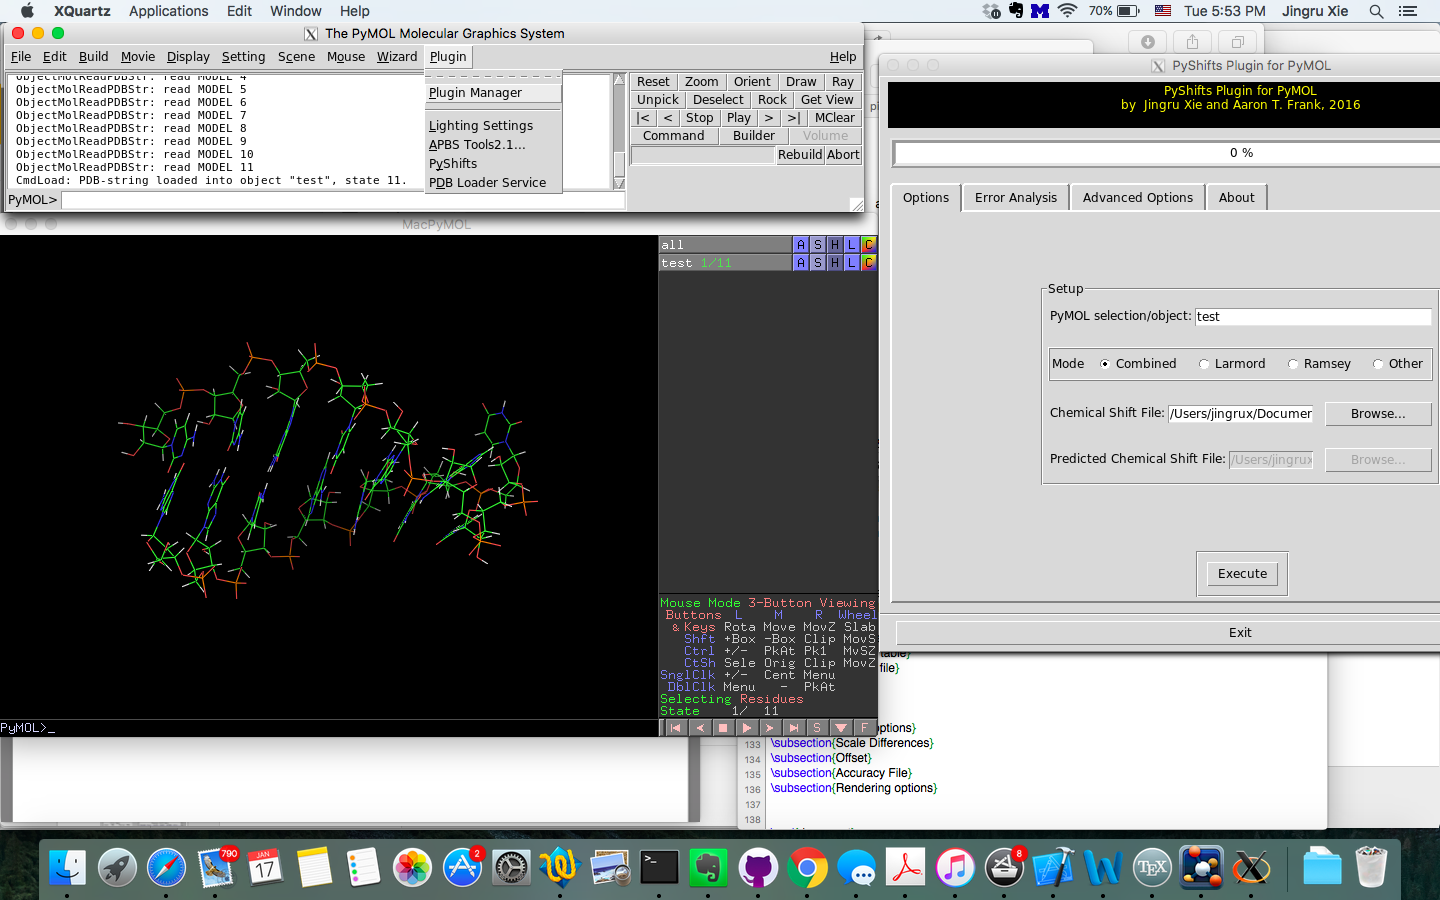
\includegraphics[width=0.7\textwidth]{layout_0.png}
\caption{Run Pyshifts from PyMOL.}
\label{fig:layout0}
\end{figure}


A new window will pop up. This is the main page of Pyshifts. Basic options will show in main page. At the top of the window is a progress bar. When running, progress bar will show the progress of your current operation. Under progress bar is the main menu bar. By clicking on those tabs you can switch back and forth among the four tabs: "Options" (default), "Error Analysis", "Advanced Options" and "About".

\begin{figure}[htbp]
\centering
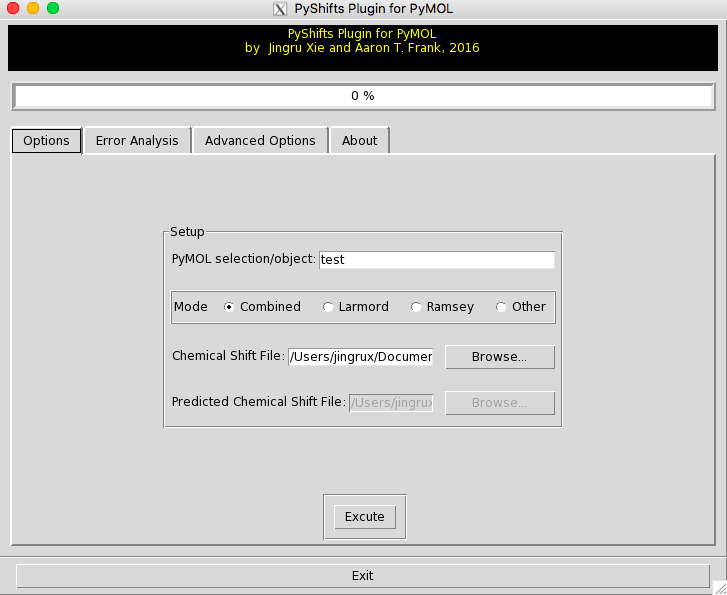
\includegraphics[width=0.6\textwidth]{main}
\caption{Pyshifts default window.}
\label{fig:layout1}
\end{figure}

\subsection{Test case}
To start with, let's first have a try on our test case. Test case is an NMR solution structure of a 14-mer hairpin RNA with cUUCGg tetraloop \href{http://www.rcsb.org/pdb/explore.do?structureId=2koc}{PDB: 2KOC}. The structure coordinates (2KOC\_test.pdb), reference chemical shifts (measured\_shifts\_2KOC.dat) and an example predicted chemical shifts file (predicted\_shifts\_2KOC.dat) are all included in "test" folder which comes with the original package. Or you can always download the "test" folder from github site \url{https://github.com/atfrank/PyShifts}.

First, load structure into PyMOL as "test". In PyMOL command line, type in
\begin{lstlisting}
load test/2KOC_test.pdb, test
\end{lstlisting}

A structure will show in PyMOL window. This is frame of 2KOC, our test case.
\begin{figure}[htbp]
\centering
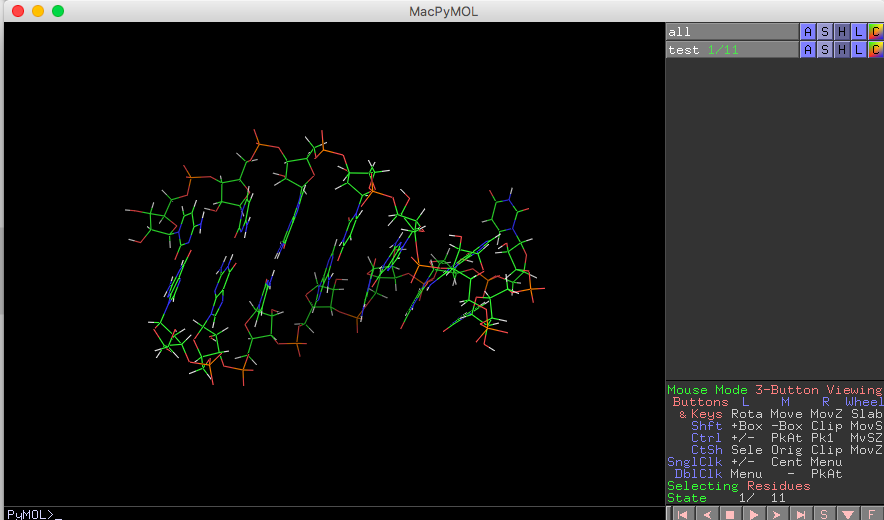
\includegraphics[width=0.7\textwidth]{test_ensemble}
\caption{Test ensemble in PyMOL.}
\label{fig:test1}
\end{figure}


\newpage
\section{Options (Setup)}

\subsection{PyMOL selection/object}
\subsection{Mode}
\subsubsection{Using predictor}
\subsubsection{Using external predicted chemical shifts file}


\newpage
\section{Error Analysis}
\subsection{Error Table}
\subsubsection{Sort table: Nuclei and Metric}
\subsection{Chemical Shifts Table}
\subsubsection{Sort table}
\subsection{Save to file}


\newpage
\section{Advanced options}
\subsection{Scale Differences}
\subsection{Offset}
\subsection{Accuracy File}
\subsection{Rendering options}


\end{document}




